\chapter{Переход Фредерикса в случае отрицательной анизотропии диэлектрической проницаемости.}\label{ch:ch4}

Ячейки ЖК с отрицательной анизотропией диэлектрической проницаемости отличаются тем, что, находясь во внешнем электрическом поле, молекулы ЖК стремятся выстроиться не вдоль его силовых линий, а поперёк.
Это связано со знаком $\varepsilon_a$: при $\varepsilon_a < 0$ энергия электрического поля в диэлектрике, даваемая формулой~\eqref{E_field}, становится минимальной, когда $\theta(z) = \pi/2$ на интервале $z\in [0,L]$.
Для анализа равновесной ориентационной структуры в ячейке ХЖК с отрицательной анизотропией диэлектрической проницаемости ($\varepsilon_a < 0$) вновь обратимся к методу численной минимизации функционала свободной энергии $\FF_\mathrm{tot}$.
Процедура минимизации функционала свободной энергии $\FF_\mathrm{tot}$ аналогична таковой, использованной в работе~\cite{OskirkoPRE2018}. 
Равновесную ориентационную структуру в ячейке ХЖК будем искать с помощью численной минимизации свободной энергии~\eqref{eq:F_for_minimization}, используя следующие значения углов лёгкого ориентирования на границах:
\begin{equation}\label{eq:initial}
	\theta_0^{(1)}=\theta_0^{(2)}={\pi}/{2},\;\phi_\mathrm{tot}^{(0)}=q_0L.
\end{equation}
Эти условия соответствуют ненапряжённому ХЖК в отсутствие внешнего электрического поля.
Сведём задачу поиска минимума функционала $\FF_\mathrm{tot}[\theta(z)]$ к задаче поиска минимума функции нескольких переменных, аппроксимировав искомую зависимость $\theta(z)$ пробной функцией
\begin{equation}\label{eq:psi+Fourier}
	\theta(z) = \pi/2 + {\delta\psi}(z,\delta_1,\delta_2) + \sum\limits_{n=1}^N c_n\sin(\pi nz/L).
\end{equation}
Здесь слагаемое $\pi/2$ соответствует неискажённому состоянию.
Функция $\delta\psi(z,\delta_1,\delta_2)$, задаваемая выражением~\eqref{psi=}, содержит $\delta_1$ и $\delta_2$ -- отклонения от углов лёгкого ориентирования на границах: $\theta(0) = \pi/2 + \delta_1$, $\theta(L) = \pi/2 + \delta_2$.
Наконец, ряд Фурье описывает объёмные искажения ориентационной структуры, не затрагивающие границы.
Используя граничные условия~\eqref{eq:gran-1}, можно выразить коэффициенты $c_N$ и $c_{N-1}$ через все остальные -- $\delta_{1,2}$ и $\{c_n\}_{n=1}^{N-2}$.
Таким образом, углы $\delta_1$, $\delta_2$, а также коэффициенты $c_n$, $n=1,\dots,N-2$ являются регулируемыми параметрами.

Ограничимся в~\eqref{eq:psi+Fourier} $N = 20$ членами ряда Фурье.
Учёт более, чем 20 слагаемых приводит к относительному изменению профиля $\theta$ менее чем на $0.5\%$ для любого $z$ на всём интервале $[0,\, L]$.
В многомерной численной минимизации существует проблема попадания в максимумы или в седловые точки.
Для того, чтобы определить, действительно ли минимизация свободной энергии привела к минимуму, используем случайные небольшие сдвиги параметров  $\delta_{1,2}$, $\{c_n\}$ относительно полученных значений.
Если минимизационный алгоритм приводит к другому ответу, это означает, что предыдущий результат был ошибочным -- максимумом или седловой точкой.
При этом в случае, если достигнут, по крайней мере, локальный минимум, то при любом достаточно небольшом сдвиге минимизация будет всегда возвращать нас обратно.

При помощи прямой минимизации свободной энергии были найдены равновесные ориентационные структуры в ячейке ХЖК при различных значениях усреднённого флексоэлектрического коэффициента $\bar{e}$ и приложенного напряжения $U$, а также следующих значениях материальных констант: $K_{11}=0.42\times 10^{-6}$~дин, $K_{22}=0.23\times 10^{-6}$~дин, $K_{33}=0.53\times 10^{-6}$~дин,  $q_0=500$~$\text{cm}^{-1}$, $L=60$~$\mu\text{m}$, $W_\theta^{(1)}=2.5\times 10^{-3}$~эрг/см$^2$, $W_\theta^{(2)}=0.5\times 10^{-3}$~эрг/см$^2$,  $W_\phi^{(1)}=2.5\times 10^{-4}$~эрг/см$^2$, $W_\phi^{(2)}=1.0\times 10^{-4}$~эрг/см$^2$, $\varepsilon_\bot=16.2$, $\varepsilon_\|=7.2$.
Заметим, что от стандартного набора параметров этот набор отличается только значениями диэлектрической проницаемости $\varepsilon_\bot$ и $\varepsilon_\|$.

Полученные результаты для $\varepsilon_a < 0$ для сравнения приводятся вместе с аналогичными результатами для $\varepsilon_a > 0$. На Рис.~\ref{fig1} на плоскости $(\bar{e},U)$ приведены рассчитанные области устойчивости планарной геликоидальной ориентационной структуры.
\begin{figure}
	\centering
	\includegraphics[width=0.49\textwidth]{1aa.eps}%{PhD_negative_ea.png}\hspace{2pc}%
	\hfill
	\includegraphics[width=0.49\textwidth]{1bb.eps}%{PhD_negative_ea.png}\hspace{2pc}%
	\caption{Фазовые диаграммы для случаев $\varepsilon_a < 0$ и $\varepsilon_a > 0$. Сплошной и пунктирной линией обозначена граница между различными "фазами" при разрывном и непрерывном переходе соответственно.
		Точечной линией обозначена асимптота межфазовой границы при $\varepsilon_a < 0$, а знаком ``$\circ$'' -- трикритическая точка.}\label{fig1}
\end{figure}
Данный результат можно получить и аналитически аналогично тому, как это было проделано, к примеру, в~\cite{OskirkoPRE2018}.


\section{Аналитическое изучение устойчивости планарной геликоидальной структуры в случае отрицательной диэлектрической проницаемости.}

Для определения устойчивости планарной геликоидальной структуры ($\theta_0(z) = \pi/2$, $\phi_0(z) = q_0 z$, $z\in[0,\,L]$) нужно изучить вторую вариацию свободной энергии на этой структуре, $\delta^2\FF_\mathrm{tot}(\theta_0,\phi_0)$. 
Вторая вариация свободной энергии в отсутствие флексоэлектрической поляризации уже была найдена в работе~\cite{VAR2013}:
\begin{multline}\label{eq:F2_on_planar_helicoidal}
	\left.\delta^2\FF_{\text{tot}}\right|_{\bar{e}=0}
	=\frac{S_{\!\bot}}{2}\bigg[\int_{0}^{L}
	\left(K_{11}(\delta\theta')^2+M\delta\theta^2+K_{22}(\delta\phi')^2\right)\, dz +\\
	+\sum_{\alpha=1,2}W_\theta^{(\alpha)}\delta\theta^2(l_\alpha)
	+\sum_{\alpha=1,2}W_\phi^{(\alpha)}\delta\phi^2(l_\alpha)\bigg],
\end{multline}
где
\begin{equation}
M = K_{33}q_0^2 - \varepsilon_a U^2/(4\pi L^2).
\end{equation}
Так как $J_1\big|_{\theta = \theta_0}=0$ и $\delta J_1\big|_{\theta = \theta_0}=0$, то вклад во вторую вариацию свободной энергии, обусловленный флексоэлектрической поляризацией, даётся выражением
\begin{equation}\label{get_d2Flex}
\delta^2\FF_{\mathrm{flex}}
=-S_{\!\bot}\bar{e} (U/L) \delta\theta^2\Big|_0^L.
\end{equation}
Следовательно, вторая вариация свободной энергии $\delta^2\FF_\mathrm{tot}=\left.\delta^2\FF_{\text{tot}}\right|_{\bar{e}=0} + \delta^2\FF_{\mathrm{flex}}$ оказывается суммой двух независимых вариаций по углам $\theta$ и $\phi$.
При этом часть, зависящая от вариации $\phi$, положительно определена, так как $K_{22}>0$ и $W^{(1,2)}_\varphi>0$.
Таким образом, устойчивость планарной геликоидальной струтктуры определяется только членами, зависящими от вариации $\theta$:

\begin{equation}\label{d2F_theta}
\delta^2 \FF_\theta =
\frac{S_{\!\bot}}{2}\int_{0}^{L}\left(K_{11}(\delta\theta')^2 + M(\delta\theta)^2\right) dz + \frac{S_{\!\bot}}{2}\sum_{\alpha=1,2}
\EuScript{W}^{(\alpha)}
\delta\theta^2(l_\alpha),
\end{equation}
где
\begin{equation}\label{W_renorm}
\EuScript{W}^{(\alpha)}=W_\theta^{(\alpha)} - 2(-1)^\alpha\bar{e} U/L.
\end{equation}
Вклад флексоэлектрической поляризации во вторую вариацию свободной энергии $\delta^2\FF_\text{tot}$ сводится к ренормированию модулей сцепления с поверхностью, $W_\theta^{(\alpha)}\rightarrow \EuScript{W}^{(\alpha)}$.
Следует отметить, что один из эффективных модулей зацепления $\EuScript{W}^{(\alpha)}$ с ростом приложенного напряжения $U$ увеличивается и остаётся положительным, в то время как другой уменьшается и при достаточно больших значениях $U$ становится отрицательным.
Введём следующие обозначения:
\begin{equation}\label{Wtheta_eff_pm}
\EuScript{W}^{+} =
\begin{cases}
\EuScript{W}^{(1)},&\mbox{if } U >0,\\
\EuScript{W}^{(2)},& \mbox{if } U<0,
\end{cases}\quad
\EuScript{W}^{-} =
\begin{cases}
\EuScript{W}^{(2)},& \mbox{if } U >0,\\
\EuScript{W}^{(1)},& \mbox{if } U<0.
\end{cases}
\end{equation}
Как следует из выражения~\eqref{d2F_theta}, планарная геликоидальная структура может стать неустойчивой только если $\EuScript{W}^{-}$ отрицательно.
Это приводит к требованию
\begin{equation}\label{eq:conditions_for_voltages}
	U_\mathrm{flex}< \left|U\right|,
\end{equation}
где
\begin{equation}\label{UfrUfl}
U_\mathrm{flex}=
\frac{L}{2\bar{e}}
\begin{cases}
W_\theta^{(2)},&\!\! \text{если } U >0,\\
W_\theta^{(1)},&\!\!\text{если } U<0.
\end{cases}
\end{equation}

Представим $\delta \theta(z)$ в виде суммы двух слагаемых:
\begin{equation}\label{thetamupsi}
\delta\theta(z) = \delta\psi(z) + \delta\mu(z),
\end{equation}
где
\begin{equation}\label{mu0=muL=0}
\delta\mu(0) = \delta\mu(L) = 0,
\end{equation}
а функция $\delta\psi(z)=\delta\psi(z,\delta_1,\delta_2)$ выбрана как решение следующего дифференциального уравнения с граничными условиями:
\begin{equation}\label{eq:diff_system}
\begin{cases}
K_{11} \delta\psi''(z) - M\delta\psi(z) = 0,\\
\delta\psi(0) = \delta_1,\ \delta\psi(L) = \delta_2.
\end{cases}
\end{equation}
Такой выбор $\delta\mu(z)$ и $\delta\psi(z)$ даёт возможность разделить интегральный член в~\eqref{d2F_theta}, на два слагаемых, по отдельности зависящих от этих функций; выполнение первого условия в~\eqref{eq:diff_system} позволяет исключить ``перекрёстный член'' после подстановки $\delta\psi(z)$ и $\delta\mu(z)$ в~\eqref{d2F_theta}.

Решение уравнения~\eqref{eq:diff_system} с учётом $\ve_a < 0$ может быть представлено в следующем виде:
\begin{equation}\label{psi=}
\delta\psi =
\displaystyle\delta_1\frac{\sinh \xi(L-z)}{\sinh\xi L}+\delta_2\frac{\sinh\xi z}{\sinh\xi L}
\end{equation}
где обратная длина $\xi$ определяется как
\begin{equation}\label{xi=}
\xi = \sqrt{\left|M\right|K_{11}^{-1}} = \sqrt{\left|K_{33}q_0^2-\varepsilon_a U^2/(4\pi L^2)\right|K_{11}^{-1}}.
\end{equation}
Разделяя $\delta\theta$ на два слачаемых, даваемых выражениями~\eqref{thetamupsi} и~\eqref{psi=}, представим $\delta^2\FF_\theta$ в виде суммы двух независимых квадратичных форм
\begin{equation}
\delta^2 \FF_\theta =\frac{1}{2}S_{\!\bot}( Q_\psi + Q_\mu),
\label{eq:separation_into_two_modes}
\end{equation}
где
\begin{eqnarray}\label{Qdelta0}
\hspace{-7mm}&&Q_\psi= \int_{0}^{L}\left(K_{11}\delta\psi'^2(z)+M\delta\psi^2(z)\right)\mathrm{d}z
+\!\sum_{\alpha=1,2}\EuScript{W}^{(\alpha)}\delta_\alpha^2,\\
\hspace{-7mm}&&Q_\mu=\int_{0}^{L}\left(K_{11}(\delta\mu')^2+M(\delta\mu)^2\right)\mathrm{d}z.\label{Qmu}
\end{eqnarray}
Стоит отметить, что только $Q_\psi$ зависит от искажений на границе $\delta_{1,2}$.
Идея такого разделения вариации на часть, зависящую от вариации функции в объёме и часть, зависящую от, в том числе, граничных вариаций, впервые была применена Фейнманом~\cite{Feynman}.
Сейчас эта идея широко используется при описании ячеек ЖК~\cite{VRR2001, Kiselev2004, VAR2013}.
Так как $K_{11}>0$ и $M > 0$, квадратичная форма $Q_\mu$ оказывается положительно определённой.
Подставляя~\eqref{psi=} в~\eqref{Qdelta0}, получаем
\begin{equation}\label{eq:Q_psi_final}
Q_\psi=
\sum\limits_{\alpha=1,2}\left(K_{11}\xi \coth{\xi L}+\EuScript{W}^{(\alpha)}\right) \delta_\alpha^2 
- 2K_{11} (\xi/\sinh\xi L)\delta_1\delta_2.
\end{equation}
Используя критерий Сильвестра для $Q_\psi$, получаем условия устойчивости планарной геликоидльной структуры ХЖК:
\begin{align}\label{eq:ineq_all_M_final}
	\begin{cases}
		w^{+}+ t\coth t>0,\\
		w^{(1)}w^{(2)}+2\bar{w}  t \coth t>- t^2,
	\end{cases}%\label{eq:ineq_M>0_final_c}
\end{align}
где введены безразмерные параметры $t = \xi L$, $w^{+}={\EuScript{W}^{+} L}/{K_{11}}$, $w^{(\alpha)}={\EuScript{W}^{(\alpha)} L}/{K_{11}}$, и $\bar{w}=({W}^{(1)}_\theta+{W}^{(2)}_\theta)L/2K_{11}$.
Видно, что первое неравенство в~\eqref{eq:ineq_all_M_final} выполнено при любых возможных значениях $t$ и $w^{+}$.
Таким образом, критерий устойчивости планарной геликоидальной структуры в случае $\ve_a < 0$:
\begin{equation}\label{stab_cond_final}
w^{(1)}w^{(2)}+2\bar{w}   t \coth t+ t^2>0.
\end{equation}
Неравенство~\eqref{stab_cond_final} трансцендентно относительно напряжения $U$, содержащегося в $t=\xi L$, где $\xi$ даётся выражением~\eqref{xi=}. Однако $\bar{e}$ входит только в $w^{(\alpha)} = \EuScript{W}^{(\alpha)}L/K_{11}$, где $\EuScript{W}^{(\alpha)}$ даются выражением~\eqref{W_renorm}.
Таким образом, неравенство~\eqref{stab_cond_final} квадратично относительно $\bar{e}$, и условия устойчивости могут быть записаны явно:
\begin{subequations}\label{eqU*analitic}
	\begin{align}
		&0\leq \bar{e}\leq+\infty,\!\!  &&\text{если }U = 0, \label{eq:interval_1}\\
		&0\leq \bar{e} < e_+^*,\!\!  &&\text{если }0<|U|<U_\infty,\label{eq:interval_2}\\
	\end{align}
\end{subequations}
где $ \Delta{w}=({W}^{(2)}_\theta-{W}^{(1)}_\theta)L/K_{11}$,
\begin{equation}\label{eq:!!}
e_{+}^*(U)=\left(K_{11}/4U\right)\left(\Delta{w}
+ 2\bar{w}\sgn{U}\sqrt{ 1+X(U) }\right) ,
\end{equation}
\begin{equation}\label{eq:e(U)_ea<0}
X(U)=\frac{2}{\bar{w}} \left(\displaystyle t\coth t +{t^2}/2\bar{w} \right),
\end{equation}
Кривая $e^*_+(U)$, построенная по выражению~\eqref{eq:e(U)_ea<0}, совпадает с расчётной кривой $U^*(\bar{e})$.
Кроме того, можно рассчитать положение вертикальной асимптоты $\bar{e}'$:
\begin{equation}
\bar{e}' = \lim_{U\to \infty} \bar{e}^*_+(U) = \sqrt{\frac{-\ve_a K_{11}}{16\pi}}
\end{equation}
Подставляя указанные выше значения параметров, получаем $\bar{e}' =2.74\times 10^{-4} $~Фр/см, что также хорошо согласуется с численными расчётами.

Отметим важные свойства диаграммы в случае $\varepsilon_a < 0$.
С одной стороны, переход Фредерикса оказывается невозможен при небольших значениях $\bar{e}$.
Этот результат, в частности, согласуется с эмпирическим представлением о том, как должны выстраиваться молекулы с отрицательной анизотропией диэлектрической проницаемости во внешнем электрическом поле в отсутствие флексоэлектрической поляризации.
С другой стороны, существует некоторое значение $\bar{e}'$ такое, что при $\bar{e} > \bar{e}'$ переход возможен, причём напряжение, необходимое для этого, убывает убывает с ростом $\bar{e}$.
Таким образом, кривая зависимости $U = U^*(\bar{e})$ имеет две асимптоты: горизонтальную $U = 0$ и вертикальную $\bar{e} = \bar{e}' =2.74\times 10^{-4} $~Фр/см.
Также отметим, что в случае $\ve_a < 0$ возможен только непрерывный переход Фредерикса.
Этот вывод можно сделать по результатам численной минимизации свободной энергии.
%На Рис.~\ref{fig1} можно увидеть довольно неожиданный результат для $\varepsilon_a<0$.
%Оказалось, что существует такое значение $\bar{e}$ (вертикальная асимптота), выше которой может существовать искажённая структура.
%Ниже этого предела искажённая фаза не может существовать ни при каком значении $U$.
На Рис.~\ref{fig2} приведены профили полярного угла $\theta(z)$, рассчитанные при фиксированном напряжении $U = 1.2$~В и различных значениях $\bar{e}$.
\begin{figure}
	\centering
	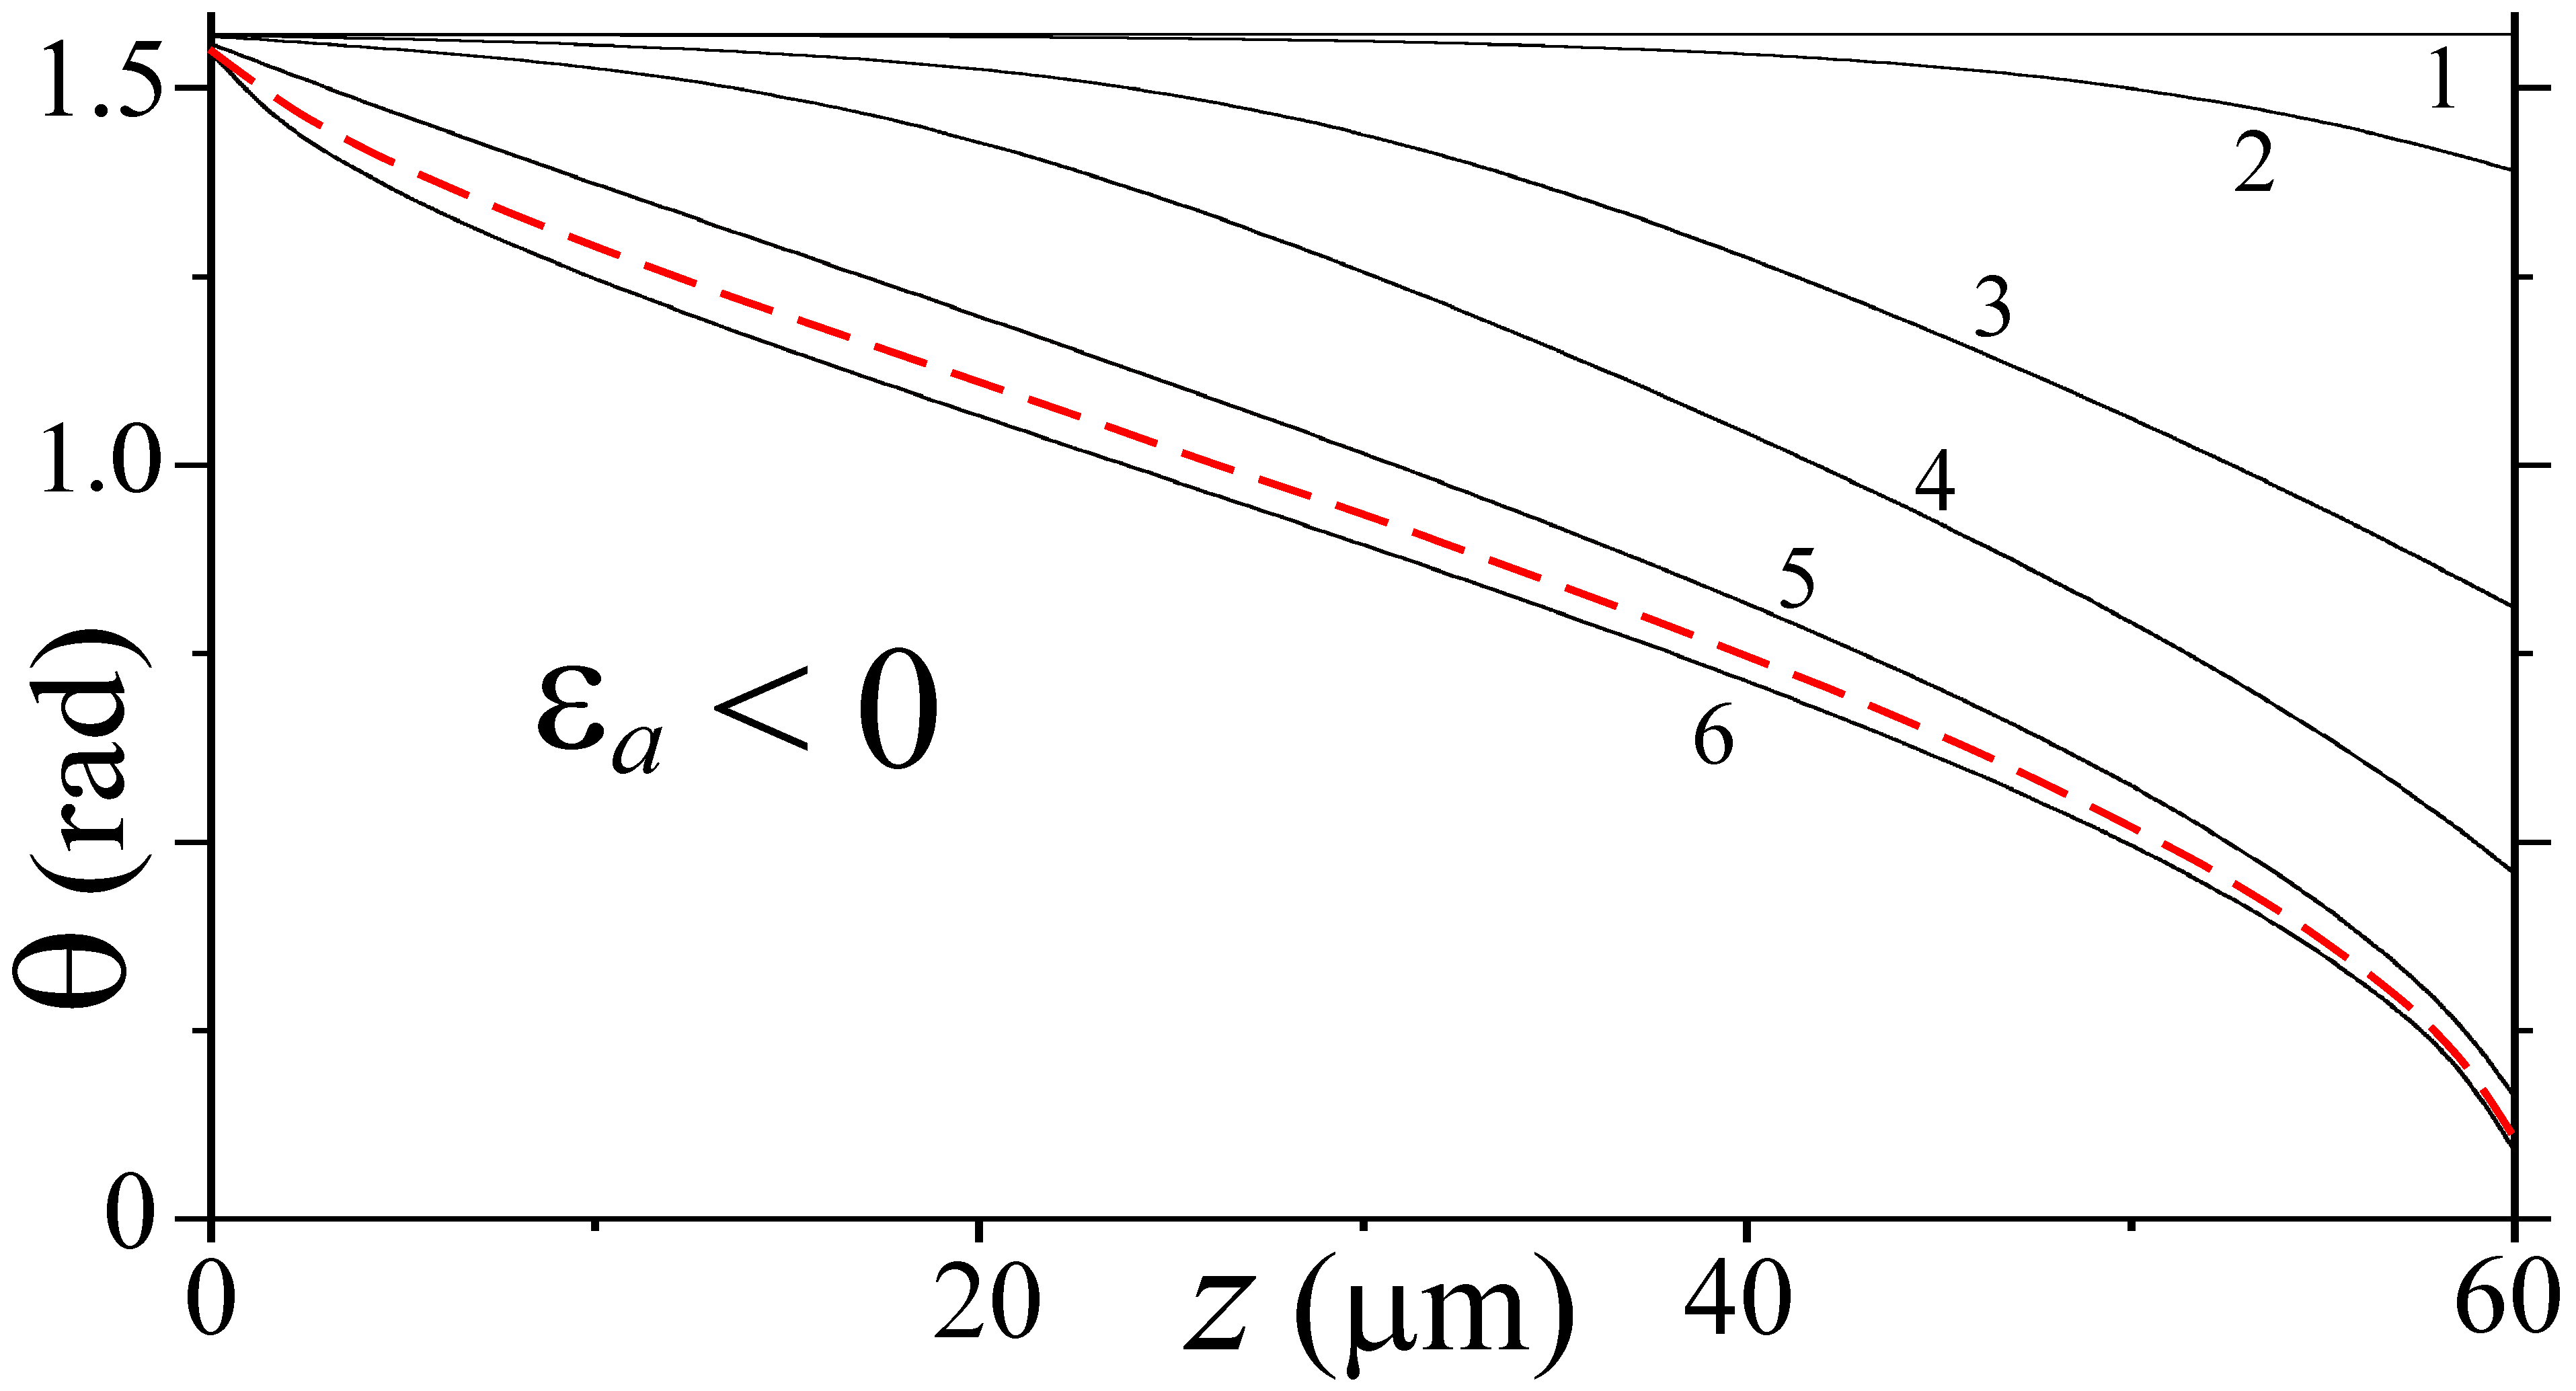
\includegraphics[width=0.49\textwidth]{Fig4_parody1a.eps}
	\hfill
	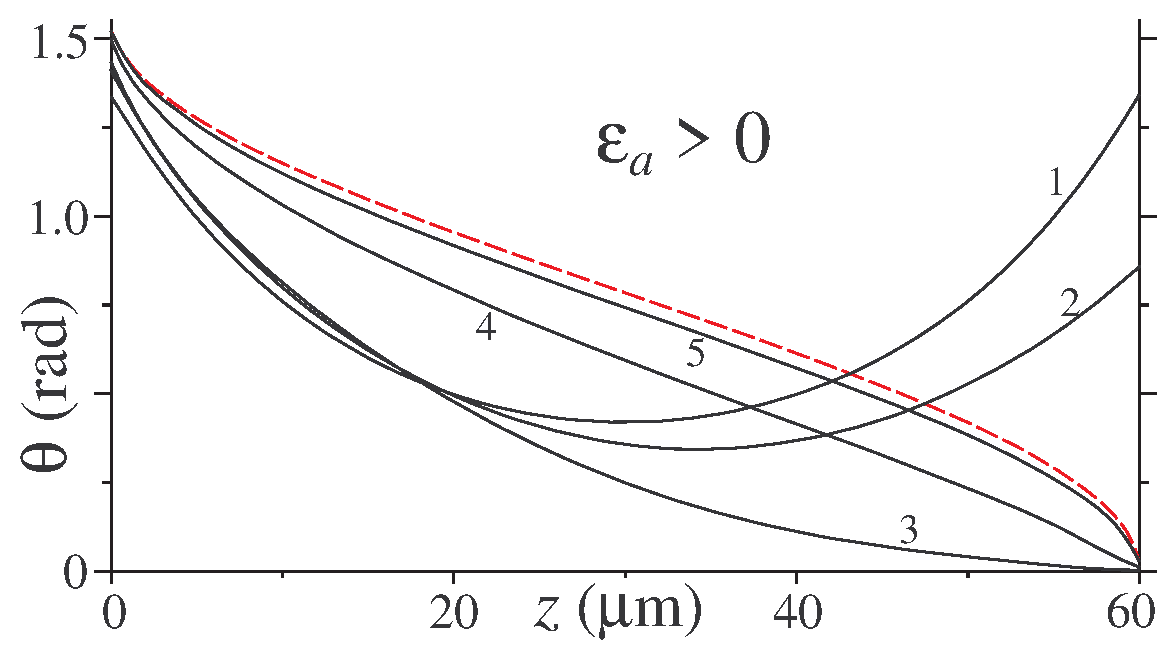
\includegraphics[width=0.49\textwidth]{symm_all_6curvesNoReflect1b.eps}
	\caption{Графики зависимости $\theta(z)$ при $U=1.2$~В.
		Значения $\bar{e}$ в единицах $\mathrm{statC/cm}$ для случая $\varepsilon_a < 0$: 1 -- $\bar{e}=10^{-3}$, 2 -- $\bar{e}=1.5\times 10^{-3}$, 3 -- $\bar{e}=1.8\times 10^{-3}$, 4 -- $\bar{e}=2\times 10^{-3}$, 5 -- $\bar{e}=3\times 10^{-3}$, 6 -- $\bar{e}=10^{-2}$; значения $\bar{e}$ при $\varepsilon_a > 0$: 1 -- $\bar{e}=0$, 2 -- $\bar{e}=10^{-4}$, 3 -- $\bar{e}=10^{-3}$, 4 -- $\bar{e}=3\times 10^{-3}$, 5 -- $\bar{e}=10^{-2}$ в единицах $\text{Фр}/\text{см}$.
		Красные пунктирные линии соответствуют зависимости $\cos^2\theta(z)\simeq {z/L}$.}\label{fig2}
\end{figure}
В случае, когда $\bar{e}$ достаточно мал, равновесные ориентационные структуры значительно отличаются для $\varepsilon_a > 0$ и $\varepsilon_a < 0$.
Однако с ростом $\bar{e}$ ориентационные структуры становятся очень схожи.
Это интересное свойство может быть объяснено следующим образом.
Выражение для свободной энергии~\eqref{eq:free-energy} при больших значениях $\bar{e}$ и/или $U$ (когда вкладами, содержащими $K_{ii}$ и $W^{(\alpha)}_{\theta,\varphi}$, можно пренебречь), сводится к следующему:
\begin{equation}\label{eq_F_f_final123}
\FF\simeq-\frac{S_{\!\bot}}{8\pi}U^2 J +S_{\!\bot} \bar{e}U JJ_1 + 2\pi S_{\!\bot} \bar{e}^2\int_{0}^{L}\frac{(\sin 2\theta \,\theta'-JJ_1)^2}{{\EE}(\theta)}dz.
\end{equation}
Рассмотрим ситуацию, когда вклады, содержащие $\bar{e}$, значительно превосходят первый вклад в~\eqref{eq_F_f_final123}.
Чтобы выяснить критерий наступления этого случая, оценим по модулю отношение второго слагаемого в~\eqref{eq_F_f_final123} к первому:
\begin{equation}\label{ch4:eq_e/U>>1}
\frac{8\pi\bar{e}UJJ_1}{U^2 J}\sim \frac{\bar{e}}{\ve_a U} \gg 1
\end{equation}
Последнее неравенство и является критерием.
Кроме того, в ситуации, когда $\sin 2\theta \,\theta'-JJ_1\neq 0$, это же неравенство означает превосходство последнего слагаемого в~\eqref{eq_F_f_final123} над остальными.
Определим, какой профиль $\theta(z)$ даёт доставляет минимум функционалу~\eqref{eq_F_f_final123}, когда выполнено условие~\eqref{ch4:eq_e/U>>1}.
Можно заметить, что интеграл в слагаемом, содержащем $\bar{e}^2$, неотрицателен, а значит, на равновесной ориентационной конфигурации $\theta(z)$ должен быть близок к нулю.
Это достигается, когда выполнено следующее равенство:
\begin{equation}
\sin 2\theta \,\theta'-JJ_1 = 0.
\end{equation}
Общим решением этого дифференциального уравнения является функция $\theta(z)$, для которой
\begin{equation}\label{ch4:eq_cos2=az+b}
\cos^2\theta(z) = az+b
\end{equation}
с произвольными константами $a$ и $b$.
Так как третье слагаемое в~\eqref{eq_F_f_final123} близко к нулю, минимум свободной энергии определяется вторым слагаемым.
Подставляя~\eqref{ch4:eq_cos2=az+b} в~\eqref{eq_F_f_final123} и опуская первое слагаемое, получаем
\begin{equation}
\FF \simeq -S_\bot \bar{e} U a.
\end{equation}
Таким образом, минимуму $\FF$ соответствует максимальное положительное значение $a$.
Для его определения учтём ограничения на $a$ и $b$, следующие из определения~\eqref{ch4:eq_cos2=az+b}:
\begin{equation}\label{ch4:eq_rectangle01}
0 \leq az + b \leq 1
\qquad \forall z\in [0,\ L]
\end{equation}
Таким образом, отрезок прямой $az+b$ на $z\in[0,\ L]$ должен целиком находиться в области, изображённой на Рис.~\ref{ch4:pic_rectangle01}, то есть его левый конец должен лежать на левой границе приведённой области, а правый -- на правой.
\begin{figure}\label{ch4:pic_rectangle01}
	\centering
	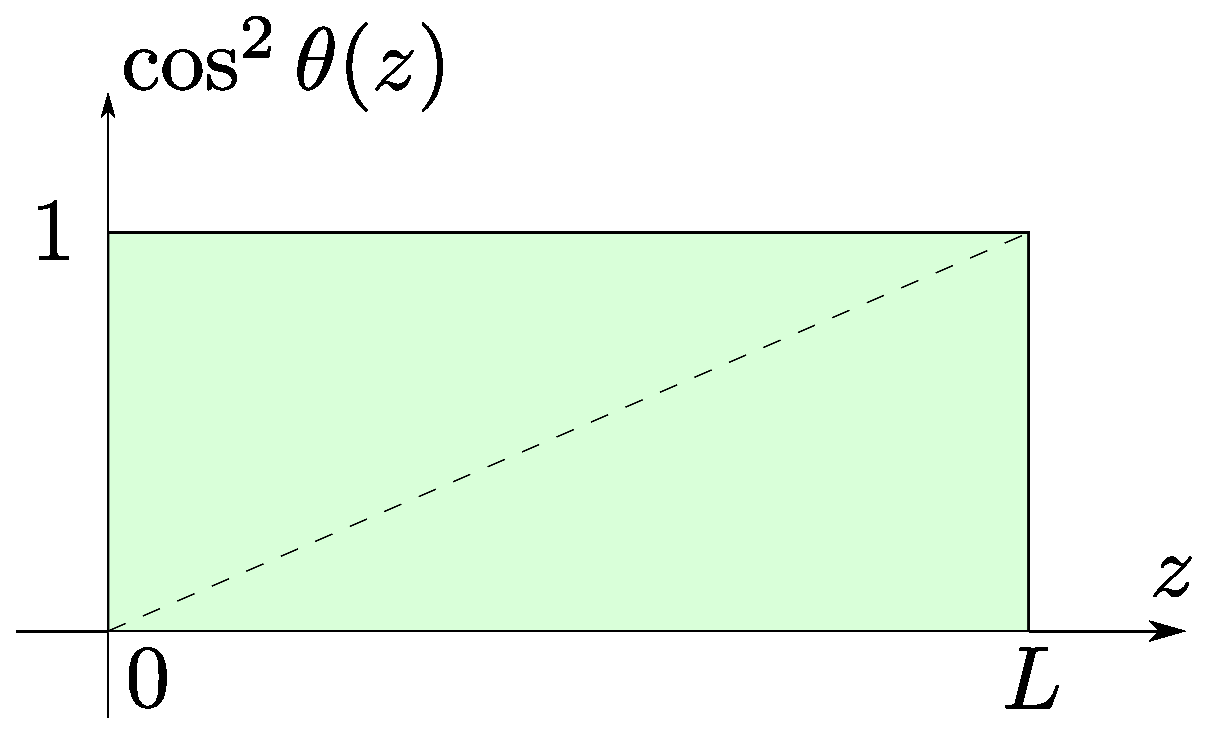
\includegraphics[width=8cm]{rectangle01}
	\caption{Область, задаваемая неравенствами~\eqref{ch4:eq_rectangle01} и отрезок прямой с наибольшим возможным угловым коэффициентом.}
\end{figure}
Нетрудно заметить, что наибольшее положительно значение $a$ соответствует прямой, отмеченной на Рис.~\ref{ch4:pic_rectangle01}  пунктиром, и равняется $1/L$, $b = 0$.
Таким образом, минимум функционала $\FF$ как при $\varepsilon_a<0$, так и при $\varepsilon_a>0$ даётся зависимостью $\cos^2\theta(z)\simeq {z/L}$.
Отметим, что при достаточно больших $\bar{e}$ равновесной является гибридно-ориентированная структура.
В такой структуре рядом с одной из границ молекулы в среднем выстраиваются параллельно ограничивающей плоскости, а рядом с другой -- перпендикулярно.
Такой переход между планарной геликоидальной и гибридной структурами может быть использован для создания переключателей, в основе работы которых лежит флексоэлектричество.

Кроме того, в ячейке ХЖК с достаточно большим $\bar{e}$ был обнаружен ориентационный переход нового типа.
Такой переход продемонстрирован на Рис.~\ref{fig4_3}, где представлены профили $\theta(z)$ при фиксированном $\bar{e}$ и различных значениях напряжения $U$.
С ростом приложенного напряжения от нулевого значения сначала происходит непрерывный переход Фредерикса.
При дальнейшем увеличении напряжения происходит ещё один переход.
Этот переход является разрывным, так как происходит между двумя значительно различающимися ориентационными структурами.
Это иллюстрируют графики 2 и 3 на Рис.~\ref{fig4_3}: разница в приложенном напряжении составляет $0.01$~В, при этом полученные профили существенно различны.
\begin{figure}
	\centering
	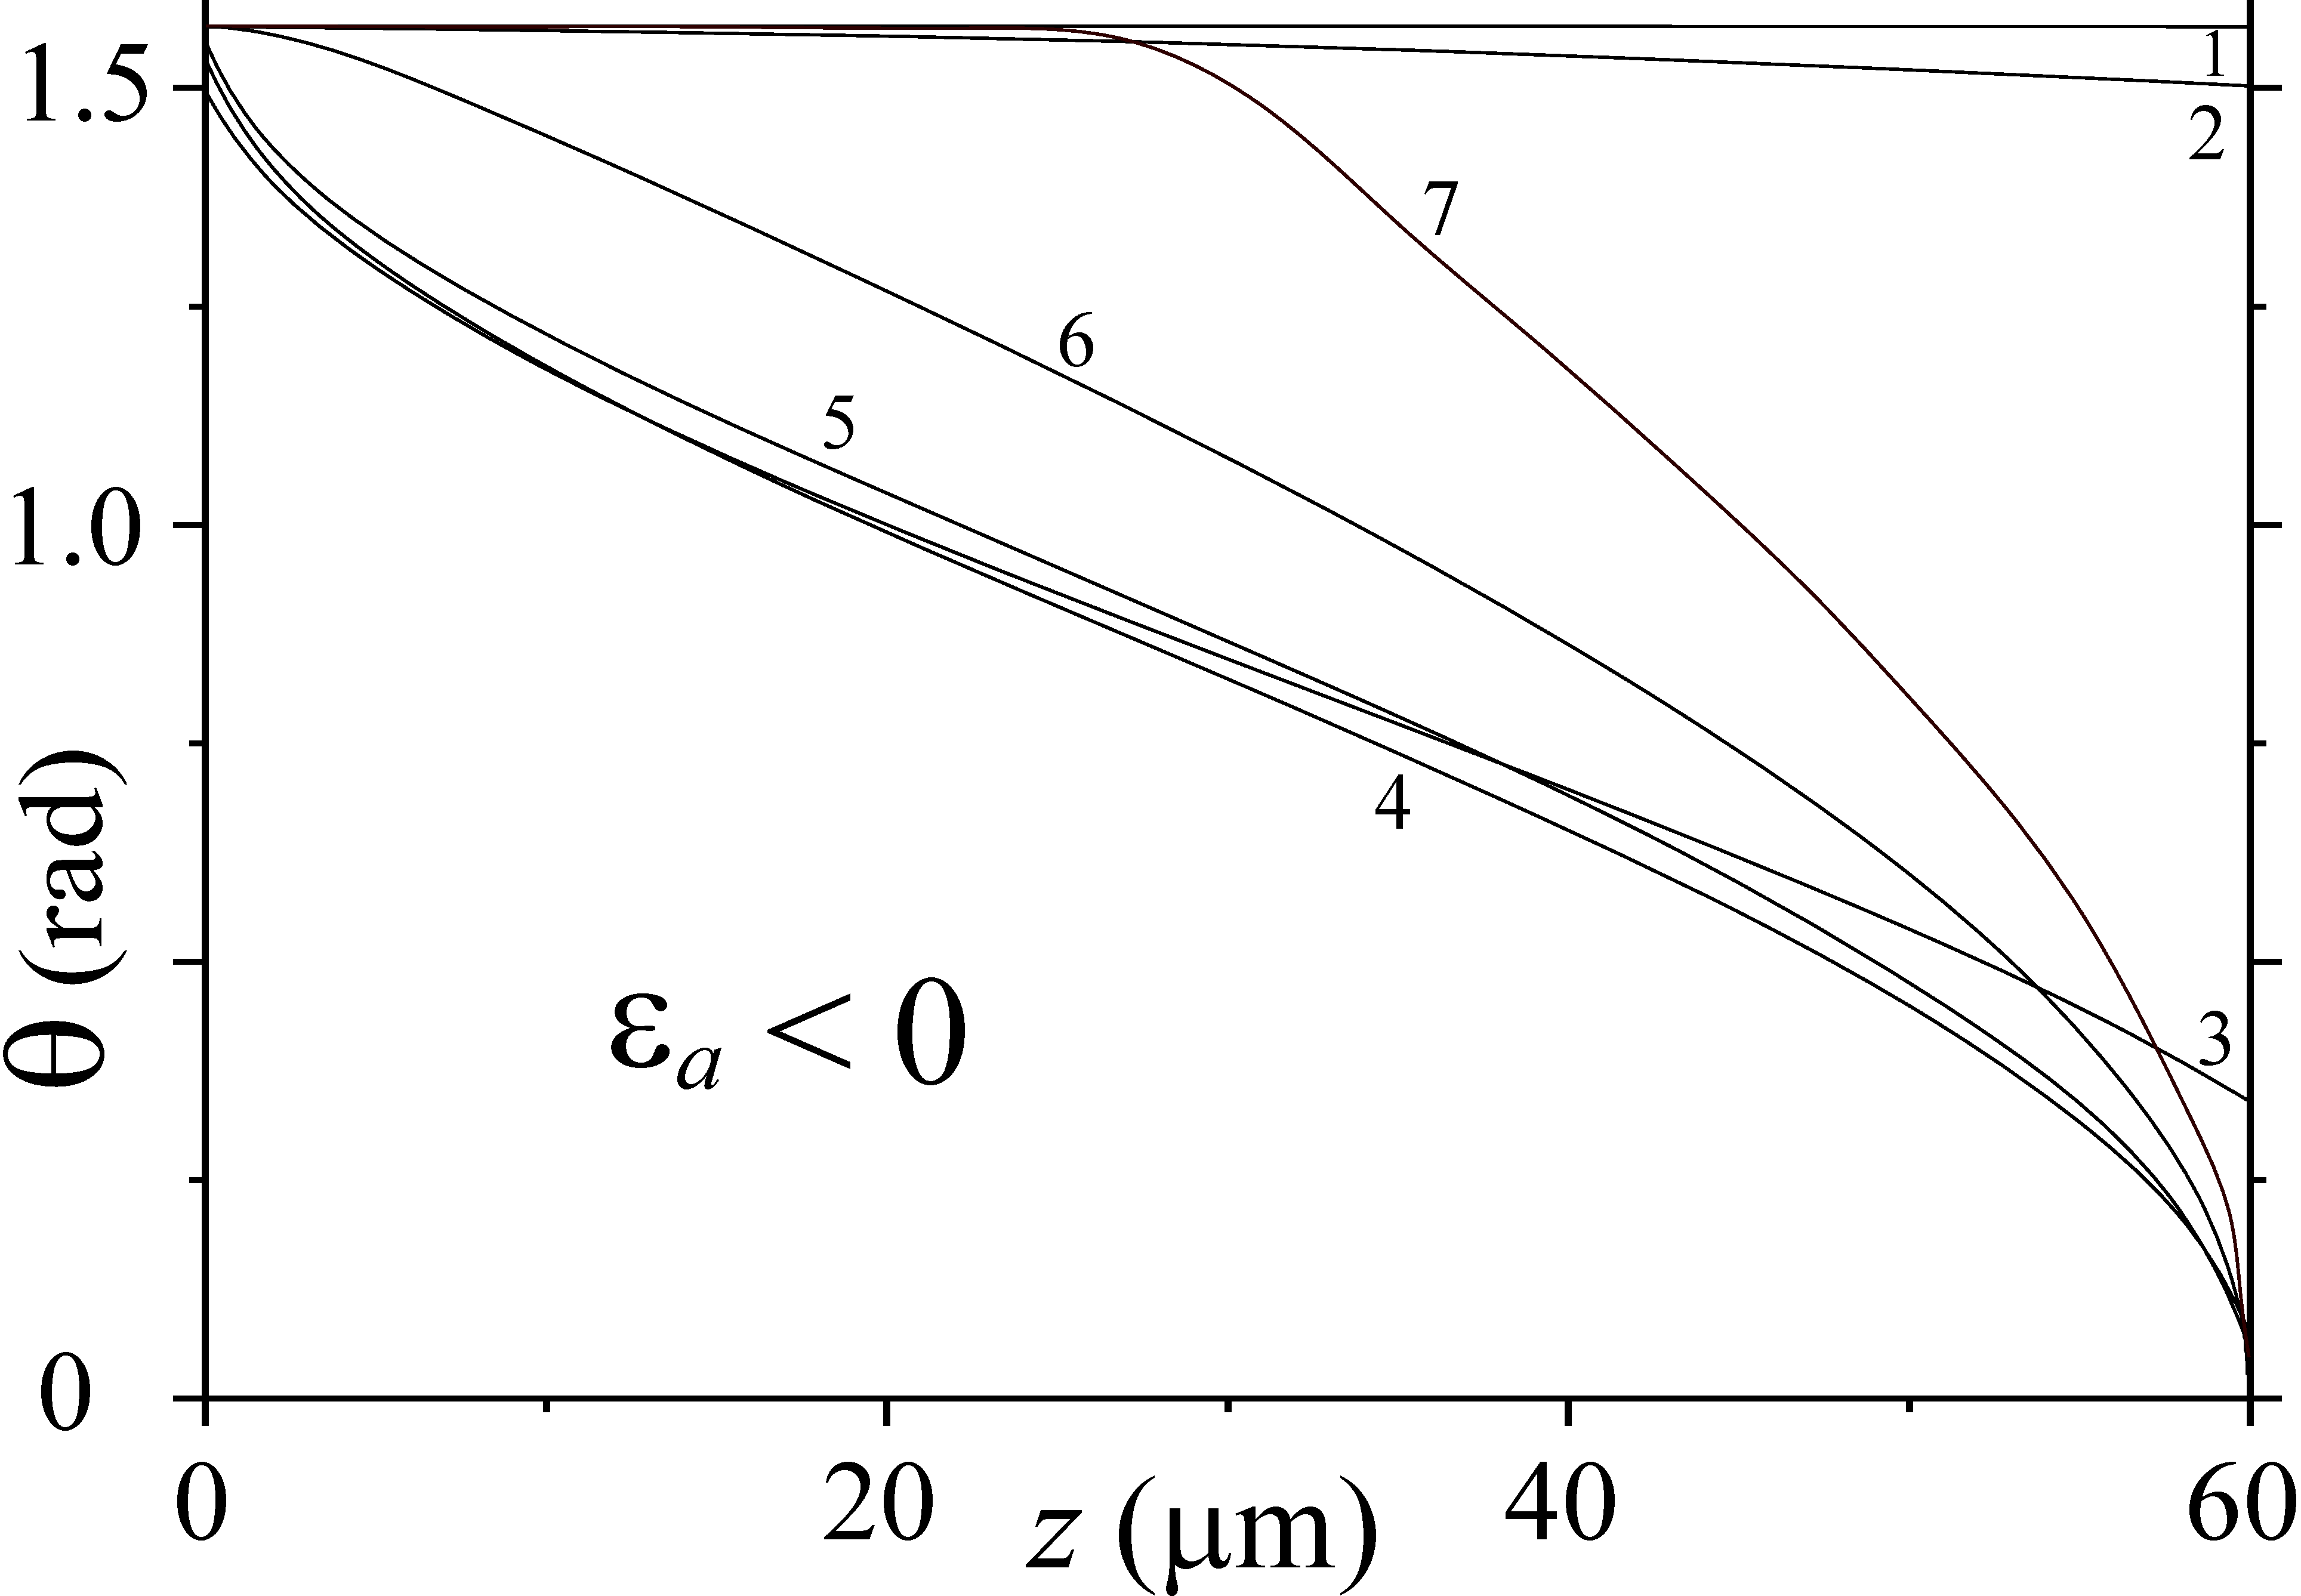
\includegraphics[width=0.48\textwidth]{Profiles_at_fixed_e_0_01_change_U.eps}%\\
	\hfill
	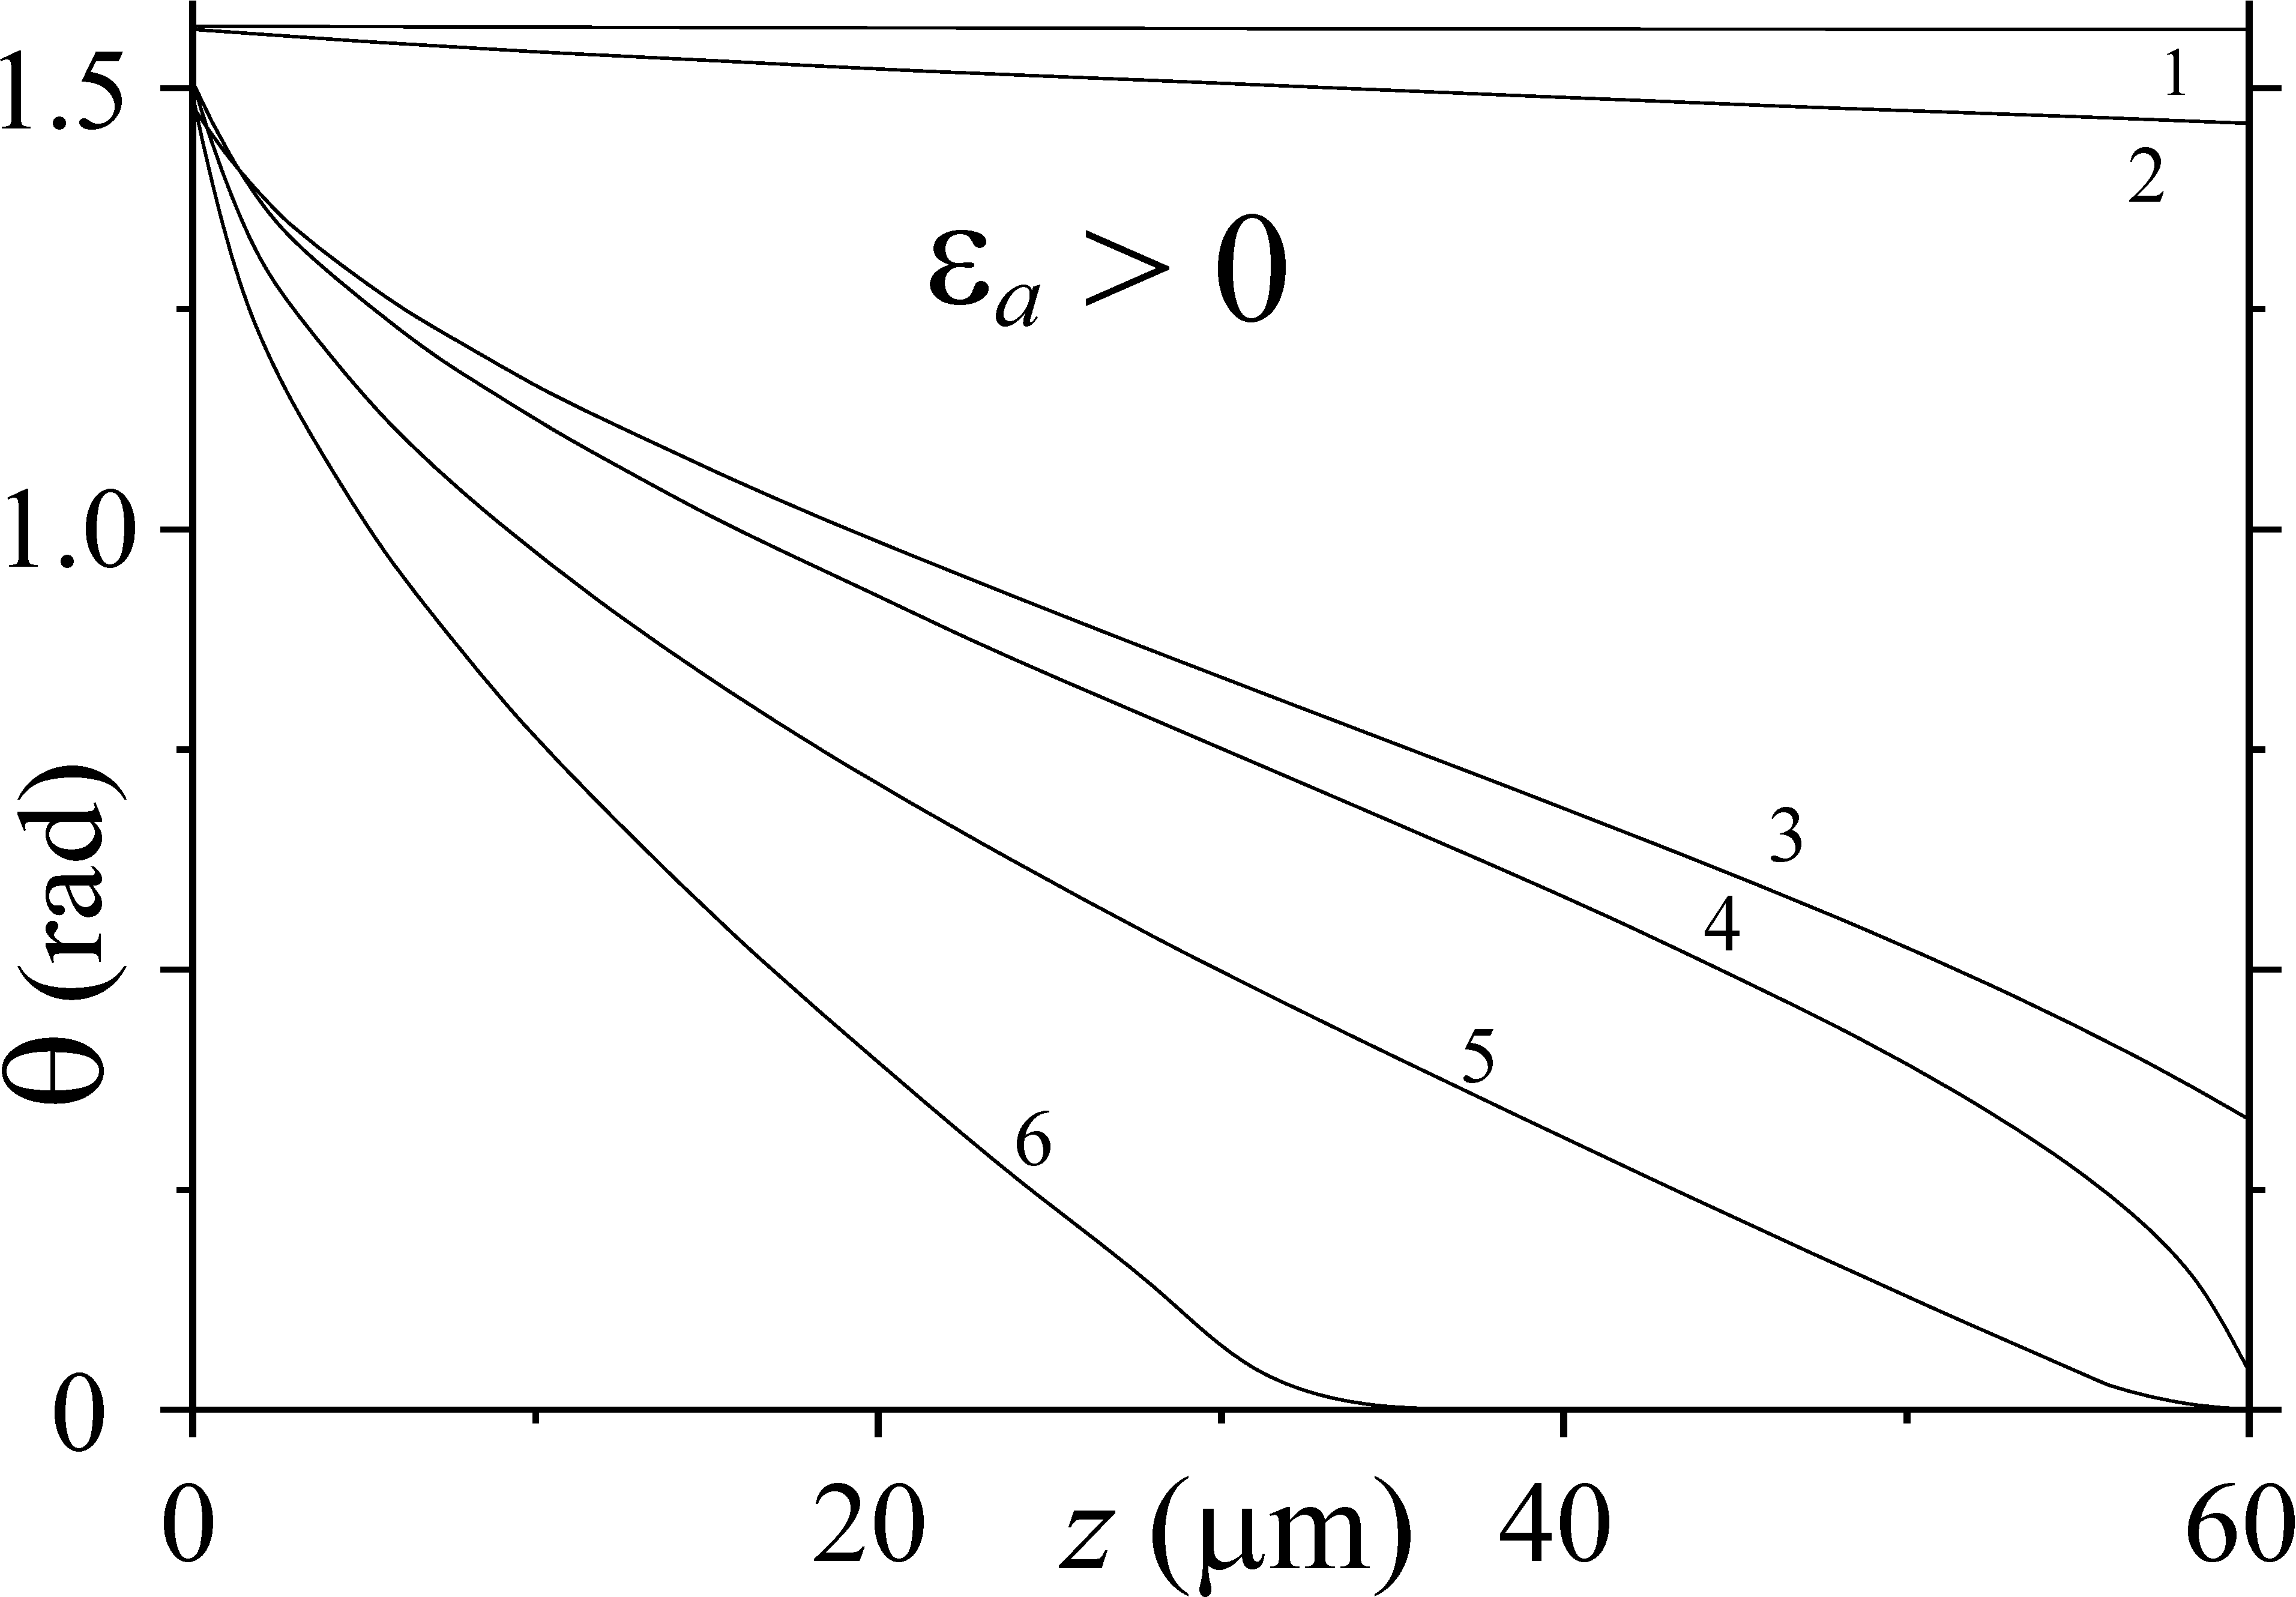
\includegraphics[width=0.48\textwidth]{Profiles_POSITIVE_EA_at_fixed_e_0_01_change_U.eps}
	\caption{Равновесная ориентационная структура $\theta(z)$ при $\bar{e}=0.01$~Фр/см. Напряжения для случая $\varepsilon_a<0$: 1 -- $U=0.15$~В, 2 -- $U = 0.17$~В, 3 -- $U = 0.18$~В, 4 -- $U = 1$~В, 5 -- $U = 2$~В, 6 -- $U = 5$~В и 7 -- $U = 10$~В; для случая $\varepsilon_a > 0$: 1 -- $U = 0.15$~В, 2 -- $U = 0.17$~В, 3 -- $U = 0.18$~В, 4 -- $U = 1$~В, 5 -- $U = 5$~В и 6 -- $10$~В.}\label{fig4_3}
\end{figure}
Отметим, что при очень высоком напряжении $U$ первое слагаемое в выражении~\eqref{eq_F_f_final123} становится определяющим.
Следовательно, система стремится к насыщенной ориентационной структуре, которая описывается зависимостью $\theta(z) = \pi/2$ при $\varepsilon_a < 0$ и $\theta(z) = 0$ при $\varepsilon_a > 0$.
Это можно пронаблюдать на Рис.~\ref{fig4_3} на примере профилей 5-7 для случая $\ve_a < 0$ и профилей 5 и 6 для случая $\ve_a > 0$.